\documentclass[11pt]{article}
%-------------------------------------------------------------------------------------------------%
\usepackage[utf8]{inputenc}
\usepackage[english]{babel}
\usepackage{biblatex}
\usepackage[a4paper, total={6in, 9in}]{geometry}
\usepackage[T1]{fontenc}
\usepackage[nottoc,numbib]{tocbibind}
\usepackage{multicol}
\usepackage{tabularx}
\usepackage{graphicx}
\usepackage{titling}
\usepackage{tocloft}
\usepackage{caption}
\usepackage{subcaption}
\usepackage{hologo}
\usepackage[hidelinks]{hyperref}
\usepackage{csquotes}
\usepackage{amsmath}
\usepackage{amssymb}
\usepackage{minted}
\usemintedstyle{emacs}
%-------------------------------------------------------------------------------------------------%
\graphicspath{ {./images/} }
\addbibresource{format.bib}
%-------------------------------------------------------------------------------------------------%
\renewcommand\cftsecpagefont{\normalfont}
\renewcommand{\cftsecleader}{\cftdotfill{\cftsecdotsep}}
\renewcommand\cftsecdotsep{\cftdot}
\renewcommand\cftsubsecdotsep{\cftdot}
\pretitle{
  \begin{center}
    \Huge\bfseries }
\renewcommand\maketitlehookb{
  \begin{center}
    \Large {An Investigatory Project Report}\\[0.25in] 
\includegraphics[scale =
      0.75]{tos_logo.jpeg}\\[0.25in] \bfseries {Submitted by}
  \end{center}
}
\predate{}
\postdate{}
\renewcommand\maketitlehookd{
  \begin{center}
    \large{ The Orchid School\\ Baner Pune 411045\\[0.3cm] \textbf{2020-2021}\\ }
  \end{center}
}
%-------------------------------------------------------------------------------------------------%
\title{RSA Encryption Tool}
\author{ Nebhrajani, Aditya V.}%\\ Magapu,Abhimanyu\\ Sharma, Galav\\ }
\date{}
%-------------------------------------------------------------------------------------------------%

\begin{document}

\maketitle
\thispagestyle{empty}

\newpage


{\center
\includegraphics[scale = 0.5]{tos_logo.jpeg}\\[0.25in]} {\center\LARGE The Orchid School\\}
{\center\huge\textbf {Certificate}\\[0.5cm]}

This is to certify that Aditya V. Nebhrajani of Class XII I1 has successfully completed the Informatics Practices
Investigatory Project in the partial fulfillment of curriculum of Central Board of Secondary
Education (CBSE) leading to award of Annual Examination of the year 2020-2021.\\[1cm]


\begin{center}
\begin{tabularx}{\textwidth}{>{\centering\arraybackslash}X  >{\centering\arraybackslash}X}
External Examiner & Teacher In-Charge \\ & (Jayashree Samudra)\\[1.5cm] Unit Head & Principal \\ (Netre
Kulkarni) & (Namrata Majhail) \\
\end{tabularx}
\end{center}

\newpage

\section*{Acknowledgements}
\addcontentsline{toc}{section}{Acknowledgements}

No project can ever be completed without the graceful contribution of many, many people.\\

I would, first and foremost, like to express my gratitude to our IP teacher, Ms. Jayashree Samudra
for her valuable advice and inputs which enhanced the quality of my work. This project could not
have been completed successfully without her help. I would also like to thank Netre Di for her
encouragement and support, and our respected principal Namrata Di for giving me an opportunity to
work on such an intriguing topic. \\

This entire project was written on open source software, using open source programming and markup
languages. I am hence deeply indebted to the open source community at large. I would like to
separately acknowledge the GNU Emacs\footnote{The Emacs text editor/eLISP REPL:
https://www.gnu.org/software/emacs/}, \LaTeX\footnote{\LaTeX\ document creation system:
https://www.latex-project.org/}, Python\footnote{Python programming language:
https://www.python.org/} and the StackExchange\footnote{StackExchange forums:
https://stackexchange.com/} communities for their powerful -- and open source -- tools.\\

Lastly, I would like to thank my parents for their love and guidance without which nothing can be
accomplished.

\newpage

\tableofcontents

\newpage
\listoffigures
\listoftables


\newpage
\section{Introduction}
Democratic governments the world over have a similar system of guaranteeing rights to people.
However, one right which is still not guaranteed by most is the right to privacy. Prior to the
advent of computer technology, privacy was easy to ensure: one had but to close the door or seal a letter.
Things have changed since then: humans communicate more and more over the Internet. This makes our
communications less private, since the medium of communication is not be secure.

In any case, there are tremendous vested interests in invading people's privacy, from showing more
personalised ads to societal control and conditioning. After whistleblower Edward Snowden leaked
the United States' National Security Agency's highly classified information, it is public domain
knowledge that not only companies but also governments invade our privacy to their own ends.

It is difficult to overstate how morally incorrect and dangerous such a practice is. Snowden put the
situation excellently:

\begin{displayquote}
  ``Arguing that you don't care about privacy because you have nothing to hide is no different than
  saying you don't care about free speech because you have nothing to say.''
\end{displayquote}

The irony of the situation is that most people are aware that companies such as Google, Microsoft and Facebook
steal their data\footnote{Reference: Ask anyone.}, but they do nothing about it. This is best
explained through consumers preferring convenience over privacy. Google is easier to use than
DuckDuckGo, and is better developed. To expect anybody other than a few highly privacy-conscious
individuals to stop using Instagram and Windows 10 is not an idea solution. Instead, the convenience
of encryption needs to be available to the general public in a user-friendly interface. Ideas like
PGP have tried and fallen into obscurity, PAKE didn't gain traction\cite{pake}, and people are
trusting, or trying to trust, WhatsApp's `end-to-end-encryption'. There is an opening for a system
that lets people secure their privacy while also being accessible and easy to
use.\cite{hackernews}\cite{gtank}

This project is an attempt to remedy this situation by building a framework for quick and easy to
use encryption. It's written in Python, which makes it easy to port or include in other
applications. The interactive CLI and Pandas database are merely for demonstration purposes.
Ideally, this project should be used as a module as part of a larger communication application.

\newpage

\section{Cryptography}

\subsection{In History}
Since time immemorial, kings, queens, and armies have relied on the privacy of their communications
to communicate battle plans to units spread over a large area. Other people reliant on privacy were
secret lovers, those inciting rebellion, and even Mary Queen of Scots.

Privacy was ensured by somehow obscuring the original message using methods such as steganography or
cryptography. Steganography is of less interest to us, as it involves physically hiding a message,
for instance, by engraving it in a hidden place. The other method, cryptography, involved taking the
original message, the `plaintext', and converting it via an algorithm to an obscure mess of letters,
the `ciphertext'. The receiver then performed the reverse algorithm and retrieved the plaintext.
Thus, even if the message were intercepted, it could not be read and its information exploited.\footnote{Image
credit: The Code Book: The Science of Secrecy from Ancient Egypt to Quantum Cryptography, Simon
Singh. OCLC: 59459928}

\begin{figure}[h]
  \centering
  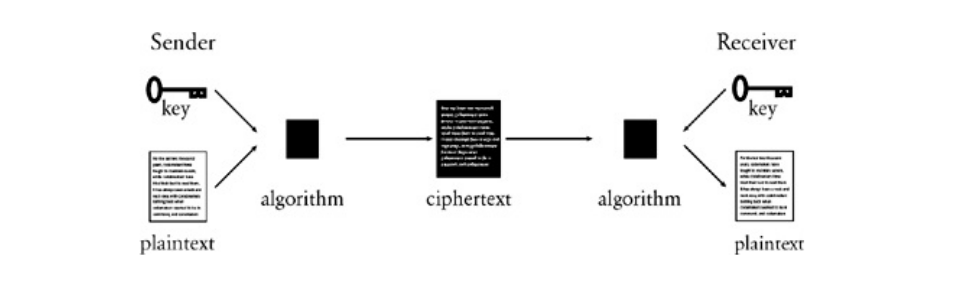
\includegraphics[scale=0.3]{cryp.png}
  \caption{Principle of encryption}
\end{figure}

In cryptography, the security of the whole system depends not on the security of the communication
medium but rather on the algorithm used. An example is the very simple Caesar cipher\cite{caesar}:

\begin{displayquote}
  The action of a Caesar cipher is to replace each plaintext letter with a different one a fixed
number of places down the alphabet. The cipher illustrated here uses a left shift of three, so that
(for example) each occurrence of E in the plaintext becomes B in the ciphertext.
\end{displayquote}

In this case, the `key' would be the number of places to shift each letter by, or the `shift'. The
Caesar cipher, like many others of its time, was broken by frequency analysis: given a long enough
sample of the ciphertext, a cryptanalyst could replace the most frequently occurring letter by the
one used most in the English alphabet (`e'), or the second most used (`t'), and so one. By trail and
error, the original message is soon revealed. In fact, the cipher of Mary Queen of Scots was broken
by frequency analysis by a cryptanalyst called Thomas Phelippes. Once the cipher was broken, the
Babington plot was revealed, and she was executed, with the cracked cipher being the central
evidence in the case against Mary Queen of Scots.

Much later, during the Second World War, the Polish and British forces joined hands to crack the
German Enigma cipher, which used an Enigma machine to encrypt the plaintext. The Polish designed
machines to crack the Enigma code (called `bombes' for the loud noises they made), which were further refined
by Alan Turing, who insisted on spending time designing mechanical machines that could break the
cipher rather than spend time cracking the ciphers by hand. This was one of the first instances of
machines being used to encrypt plaintext, and with Turing, machines being used to break ciphers.


\subsection{Modern Methods and Some Mathematics}
The primary problems in cryptography are key distribution and the security of the ciphertext. While
the security of the ciphertext can, in theory, be ensured by using complicated algorithms
implemented by machines, the problem of secure key distribution remains. If the keys are distributed
through an insecure communication medium, this renders the algorithm a mere computational hurdle at
best.

\subsubsection{Diffie-Hellman Key Exchange}
To solve the problem of secure key-distribution, Diffie, Hellman, and Merkle created a method for
generating keys even on an insecure communication medium. \cite{diffie} The method is shown in
the figure below.\footnote{Image credit: Diffie-Hellman key exchange - Wikipedia/Wikimedia Commons}

\begin{figure}[h]
  \centering
  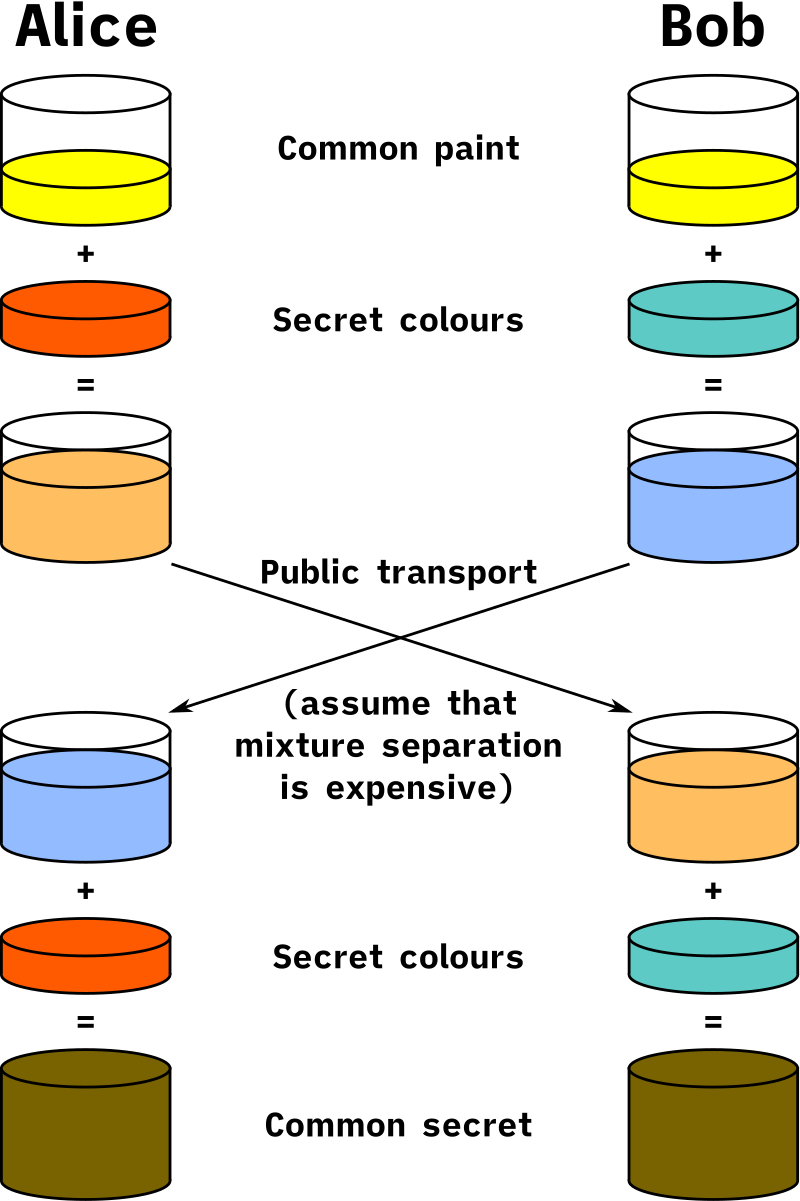
\includegraphics[scale=0.15]{diffie.png}
  \caption{Diffie-Hellman key exchange}
\end{figure}

As evident from the figure, a man-in-the-middle, despite having knowledge of the starting color
Alice and Bob agree on (yellow), and the intermediaries that they exchange (orange-tan and light
blue), he cannot find the final key since Alice and Bob do not exchange information about the secret
colors they use (blue and orange). In practice, of course, Alice and Bob use large numbers and the
modulo function (modulus from clock math) to eventually get the same secret key, which is a large
integer. This algorithm, proposed in 1976, is used to generate secret keys throughout the
Internet.  A simple generalisation of the principle used (using finite cyclic groups) is as follows
(a cyclic group is generated by a single element, and any element in the group can be obtained
by repeated group operations. A clock with an arithmetic of addition defined is a cyclic group of
order 12.):

\begin{enumerate}
\item Alice and Bob agree on a finite cyclic group $G$ (multiplicative) of order $n$ and a generating element $g$ in $G$. ($g$ is assumed to be known by all attackers.)
\item Alice picks a random natural number $a$ ($1 < a < n$) and sends $g^a$ to Bob.
\item Bob picks a random natural number $b$ ($1 < b < n$) and sends $g^b$ to Alice.
\item Alice finds $(g^b)^a$.
\item Bob finds $(g^a)^b$.
\item Since $(g^b)^a = (g^a)^b = g^{ab}$, both Alice and Bob have the same group element, which
  serves as the secret key.
\end{enumerate}


We note, however, that it is likely organisations with large budgets can crack Diffie-Hellman,
especially ones that use keys of 1024-bit lengths or less. Moreover, other vulnerabilities have been found in
Diffie-Hellman, as described in the paper \emph{Imperfect Forward Secrecy:
How Diffie-Hellman Fails in Practice}. \cite{imperfect} According to Adrian et al. around two-thirds
of popular HTTPS sites allow TLS using Diffie-Hellman and 1024-bit-keys. Some even allow legacy
512-bit keys. Two-thirds of the HTTPS servers analyzed also use common groups for generation,
meaning some primes are more `popular' than others. These vulnerabilities were exploited by the
paper and the Logjam attack was used to cryptanalyze Diffie-Hellman.

Diffie-Hellman inspired a much more powerful algorithm, the RSA asymmetric key encryption.

\subsubsection{RSA Encryption}
RSA encryption, named after Ron \textbf{R}ivest, Adi \textbf{S}hamir, and Leonard \textbf{A}dleman,
uses the concept of each user having two keys: one public key and one private key. Assume these keys
are pre-generated. Say Bob wants to send a message $M$ to Alice. Alice's public key is a tuple of
integers $(n, e)$ and her private key is an integer $(d)$. The public key is available to everyone, maybe Alice
even keeps it in her Instagram bio.
\begin{enumerate}
\item Bob converts his message $M$ into an integer $m$ using a pre-decided scheme (specified by a
  standard such as PKCS\#1).
\item Bob gets Alice's public key, $(n, e)$ and computes $$m^e \equiv c \pmod{n}$$ He then sends
  Alice $c$ over the communication medium.
\item Alice recovers $m$ from $c$ by using her private key $d$, thus: $$c^d \equiv (m^e)^d \equiv m \pmod{n}$$
\item Alice then reverses the message-to-integer scheme and gets $M$ from $m$.
\end{enumerate}

This method results in only two pieces of information passing through the communication channel:
Alice's public key, and the encrypted message, as shown in figure.\footnote{Image credit: Jin Kyu
  Lim, Medium https://medium.com/@jinkyulim96/algorithms-explained-rsa-encryption-9a37083aaa62}

\begin{figure}[h]
  \centering
  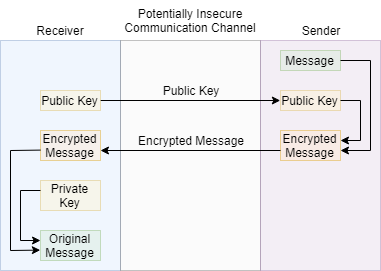
\includegraphics[scale=0.5]{rsa.png}
  \caption{RSA encryption}
\end{figure}

\paragraph{Key Generation} Keys are generated using two large primes, and this is what offers RSA
its high level of security once encrypted. The exact procedure is as follows:

\begin{enumerate}
\item Choose two distinct primes $p$ and $q$, at random. These are kept secret.
\item Compute $n = pq$. $n$ is used as the modulus, and its length expressed in bits is defined as
  the ``key length''. $n$ is part of the public key tuple.
\item Compute $\lambda (n)$, where $\lambda$ is Carmichael's totient function. Since $n=pq$,
  $$\lambda (n)  = \mathrm{LCM}(p-1, q-1)$$ $\lambda (n)$ is kept secret.
\item Choose integer $e$ such that $e$ and $\lambda (n)$ are coprimes. $e$ is usually set to
  $2^{16}+1 = 65537$, since it has a low Hamming weight (its binary representation has a lot of
  zeros). $e$ is called the public exponent.
\item Find $d$ by solving $$d\cdot e \equiv 1 \pmod{\lambda(n)}$$ that is, taking the modular multiplicative
  inverse of $e \pmod{\lambda(n)}$. $d$ is the private key and is kept secret.
\end{enumerate}

We hence have the public key tuple $(n, e)$ and the private key $d$. The above operations are
usually carried out using various optimized algorithms, which will be discussed while implementing
the Python code.

\subsubsection{RSA Proof and Example}
\paragraph{Fermat's Little Theorem}
Fermat's Little Theorem states that $a^{p-1} \equiv 1 \pmod{p}$ for any integer $a$ and prime $p$
not dividing $a$.

\paragraph{RSA Proof}
We are to show, $$(m^e)^d \equiv m \pmod{pq} \forall m$$ where $p$ and $q$ are distinct primes, and
$e$ and $d$ are positive integers satisfying $$ed \equiv 1 \pmod{\lambda (pq)}$$

Since $\lambda (n)  = \mathrm{LCM}(p-1, q-1)$, by construction, divisible by both $p-1$ and $q-1$:
$$ed - 1 = h(p-1) = k(q-1)$$ for some natural numbers $h$ and $k$.

From the Chinese Remainder Theorem,
\begin{displayquote}
  To check whether two numbers, like $m^{ed}$ and $m$, are congruent mod $pq$, it suffices (and in fact is equivalent) to check that they are congruent mod $p$ and mod $q$ separately.
\end{displayquote}

To show $m^{ed} \equiv m \pmod{p}$, we consider two cases:
\begin{enumerate}
  \item If $m \equiv 0 \pmod{p}$, $m$ is a multiple of $p$ (multiplicative cyclic group). Thus,
    $m^{ed}$ is a multiple of $p$. Thus, $m^{ed} \equiv 0 \equiv m \pmod{p}$.
  \item If $m \not\equiv 0 \pmod{p}$, $$m^{ed} = m^{ed-1}m = m^{h(p-1)}m \equiv 1^hm \equiv m
    \pmod{p}$$ where $m^{h(p-1)} \equiv 1^hm \pmod{p}$ by Fermat's Little Theorem.
\end{enumerate}

We proceed similarly for $q$, which completes the proof.

\paragraph{RSA Example}
The following is a simple proof of concept of RSA.
\begin{enumerate}
\item Let $p=11$, $q=3$.
\item $n=11 \times 3 = 33$
\item $\phi = (p-1)(q-1) = 20$. Note that we're not taking the LCM. \footnote{We are using Euler's
    rather than Carmichael's totient function. Any $d$ satisfying the former satisfies the latter,
    however, sometimes, Euler's yields a $d$ larger than required. In this case, the distinction is
    irrelevant. This doesn't matter for implements that use the Chinese Remainder Theorem, as $d$ is
    not used directly.}
\item Choose $e=3$.
\item Find $d$ such that $ed \equiv 1 \pmod{\phi}$. By trial and error, $d = 7$.
\item Hence, the public key is $(33, 3)$ and the private key is 7.
\item Let us encrypt $m=7$. $$c \equiv m^e \equiv 7^3 \equiv 343 \pmod{33} = 13$$ The ciphertext is
  hence 13.
\item Now, decrypting, $$m \equiv c^d \equiv 13^7 \pmod{33} = 7$$ We hence retrieve the original message.
\end{enumerate}

\newpage

\section{Python Implementation}
We now focus on building a complete RSA system in Python (3.6) that is capable of generating keys,
maintaining a database of users and their public/private keys, and encrypting and decrypting ASCII
text files of arbitrary length in reasonable time.

Wherever further mathematics is required for implementing a certain primitive or algorithm, it is
discussed prior its implementation in code.

\subsection{Installation}
The source code for this project is available on GitHub. You should either download it from
\url{https://github.com/nebhrajani-a/rsa-py} or clone it into a new directory.
\begin{verbatim}
$ git clone https://github.com/nebhrajani-a/rsa-py ./rsa-py
\end{verbatim}

\subsubsection{Dependencies}
The major non-standard dependancy is \texttt{progress}, which draws the progress bars during
encryptions and decryptions.
\begin{verbatim}
$ pip install progress
\end{verbatim}

Other dependancies are Python 3 (note that this program will \textbf{not} run on Python 2), math
(for the ceiling function), Secrets (secure random number generation), getpass (secure password
entry) and Pandas (database management).

\subsubsection{Compatibility}
This program is written to be platform independent, using Python implementations everywhere rather
than (possibly simpler) alternatives like command line calls. It's been tested on a machine running
Linux Mint 19.3 (XFCE 64-bit) and in two Microsoft Windows virtual machines (7 and 10), and behaves
as expected. If you think you are experiencing bugs, please write an email to \href{mailto:
aditya.v.nebhrajani@gmail.com}{aditya.v.nebhrajani@gmail.com}.


\subsubsection{Executing}
To use the program, \texttt{cd} to \texttt{/src} and execute
\begin{verbatim}
$ python main.py
\end{verbatim}


\textbf{Note:} If you use Windows, Python may be aliased to \texttt{py} instead. Make sure \texttt{python} runs Python 3 and not Python 2. On some Linux systems
Python 3 needs to be called using \texttt{python3}.


\subsection{Key Generation}
To generate keys, we must have: a large prime generator for $p$ and $q$, and math functions for
taking the LCM and modular multiplicative inverse of two numbers.

\subsubsection{Large Prime Generation}
Large prime generation is a mathematics problem as there is no evident pattern to finding primes.
$\pi(n)$ is the prime counting function for primes $\leq n$. According to the prime number
theorem\footnote{Which describes the asymptotic distribution of primes in the natural numbers. In fact, it is more explicitly stated as $\lim_{x\to\infty} \frac{\pi(x)}{x/ \ln{x}} = 1$.}
$$\pi(n) \sim \frac{n}{\ln{n}}$$

or the probability of a random $n$ being prime is $1/ \ln{n}$. For instance, the probability of a
random 2048 bit number being prime is $1/ \ln{2^{2048}} \approx 1/1419$.

\paragraph{Immediate Improvements} We can improve the previously calculated probability by noting
that no prime other than two is a multiple of two, meaning we have to check only half of the
otherwise required 1419 numbers, so $\sim 710$ numbers must be checked.

Now, to check if a number is prime, we need to divide it by every divisor $d$ such that $1 < d < n$.
There's another improvement here: we only have to check till $\sqrt{n}$ since if $n$ is composite and
equal to $pq$, either $p \leq \sqrt{n}$ or $q \leq \sqrt{n}$.

Or, in Python:
\begin{minted}{python}
def prime_generator(n):
    if n % 2 == 0:
        return False
    for i in range(3, sqrt(n), 2):
        if n % d == 0:
            return False
    return True
\end{minted}

This function certainly works, but has a time complexity $\mathcal{O}(\sqrt{n})$. This will need to
be faster for generating primes as large as 2048 bits. We hence turn to the probability based
Miller-Rabin primality test.

\paragraph{Non-Trivial Square Roots} We first define trivial and non-trivial square roots. The
trivial square roots of 1 $\mod{p}$ are 1 and $-1$, as they always return 1 on being squared modulo $p$, where
$p$ is a prime satisfying $p>2$.

We define a non-trivial square root of 1 $\mod{p}$ as any root other than 1 and $-1$. We prove now
that if such a root exists, $p$ cannot be prime (a special case of the result that, in a field, a
polynomial has as many zeros as its degree).

$$x^2 \equiv 1 \pmod{p}$$ $$(x-1)(x+1) \equiv 0 \pmod{p}$$

Which means $x \equiv 1$ or $-1 \pmod{p}$.

For example, consider $3^2 = 9 \equiv 1 \pmod{8}$, meaning 3 is a non-trivial square root of 1
$\mod{8}$. Clearly, 8 is composite.

\paragraph{Miller-Rabin Primality Test}
The Miller-Rabin test relies on finding nontrivial square roots of 1 $\mod{n}$.

Let $n$ be a prime and $n>2$. $n-1$ must be even, and we write it as $2^s\times d$, where $s$ and
$d$ are positive integers and $d$ is odd. For each $a$ in $(Z/nZ)\times$ (in range $[2, n-2]$),
either $$a^d \equiv 1 \pmod{n}$$ or $$a^{2^r\cdot d} \equiv -1 \pmod{n}$$ for some $0 \leq r \leq
s-1$. To prove the claim, check that by Fermat's Little Theorem, $a^{n-1} \equiv 1 \pmod{n}$. Hence,
if we repeatedly take the square roots of $a^{n-1}$, we will get either 1 or $-1$.

The Miller-Rabin test is the contrapositive of the above, that if we can find an $a$ such that both
of the above hold false, $n$ must be composite. $a$ is called a witness to the fact that $n$ is
non-prime. If some $a$ does not satisfy the negation of both the above, $a$ is called a strong liar,
and $n$ is a strong \emph{probable} prime for base $a$ (that is, it might yet be composite and still
hold the contrapositive).

Every odd composite number $n$ has many witnesses $a$, however, if we're unlucky, $a$ will be a strong
liar for $n$ and we'll categorize it as prime. There's no known way of generating an $a$ which isn't
a liar. We instead make the test probability based: we choose a random non-zero $a$ and test it.
Since it might be a strong liar, we repeat the test for a different value of $a$. The greater the
number of iterations we check, the higher is the probability of generating a prime $n$.

\paragraph{Final Implementation} We first generate a random number $n$ using Python's
\texttt{secrets} module. \footnote{The \texttt{random} module is not suitable for cryptographic
applications. Secrets instead calls the system's most random generator, such as /dev/random on
Linux.} We first implement a low level checker:

\subsubsection{Mathematics Functions}
\subsubsection{Putting It Together}

\subsection{Primitive RSA Encryption and Decryption}
\subsubsection{Chinese Remainder Algorithm for Fast Decryption}

\subsection{ASCII to Integer via Octet Streams and Back}
\subsubsection{PT2OS}
\subsubsection{OS2IP}
\subsubsection{I2OSP}
\subsubsection{OS2PT}
\subsubsection{Putting It Together}

\subsection{File Chunking}

\subsection{User Data Pandas DataFrame}

\subsection{Interaction Functions}

\subsection{Putting It All Together}

\newpage

\section{Experiment}

\newpage

\section{Results}

\newpage

\section{Author's Note}

This paper is written as a submission to the Central Board of Secondary Education (India) as a
Informatics Practices Investigatory Project for the year 2020-21. \\
It was noticed by the author of this paper that generally, investigatory projects, which are an
amazing opportunity to showcase research and academia-related talent, typically end up being
plagiarised experiments from textbooks or the World Wide Web. In fact, the top ten results of
an Internet search for this very project: `determination of caffeine content in tea samples', are all
nearly identical papers, with the same content and errors. I hence perceive that on a general
basis, students' participation is lacking in investigatory projects.\\
This paper is an attempt to fully utilize the opportunity gracefully granted to me by CBSE and The
Orchid School, and to raise the bar for all students. It is my hope that this will inspire new and
fruitful research at the secondary level of education.\\
It has been my attempt to write this paper in the same way as a scholarly article insofar as I
could. If there are any errors or discrepancies, they remain my own.\\
I thank you for taking the time to go through this paper, and I hope you enjoyed reading it as much
as I enjoyed writing it.\\

\newpage

\printbibliography
\addcontentsline{toc}{section}{References}
\end{document}
